\documentclass{article}
\usepackage{amsmath, amssymb, bm, booktabs, tabularx, tikz}
\usepackage{afterpage}
\usepackage{nicematrix}
\usetikzlibrary{arrows.meta, positioning}
\title{Kalman Filter State Estimation for Blue Jay Racing 23xt}
\author{Nikhil Mani}

\begin{document}

\maketitle
\tableofcontents
\section{Introduction}

This project is going to attempt to apply a Kalman filter-based approach to perform state estimation on the Blue Jay Racing 23xt. The end goal is for us to be able to produce 3D simulated replay of each race with accurate measurements of the position, velocity, and other dynamics at each point in time. 

\section{What is a Kalman Filter?}

A Kalman filter is an ``optimal filter,'' or a state estimation method that has formal guarantees on optimality in specific situations. The general idea of a Kalman filter is to condition your estimate of the system on your observations—and the variance associated with them-to get a better picture of the state. They do an extremely good job of sensor fusion for state estimation, so are used widely in autonomous navigation scenarios. Kalman filters also thrive in linear systems with Gaussian noise distributions.

On a high level, the Kalman filter works like this:
\clearpage
\begin{figure}[htbp]
\centering
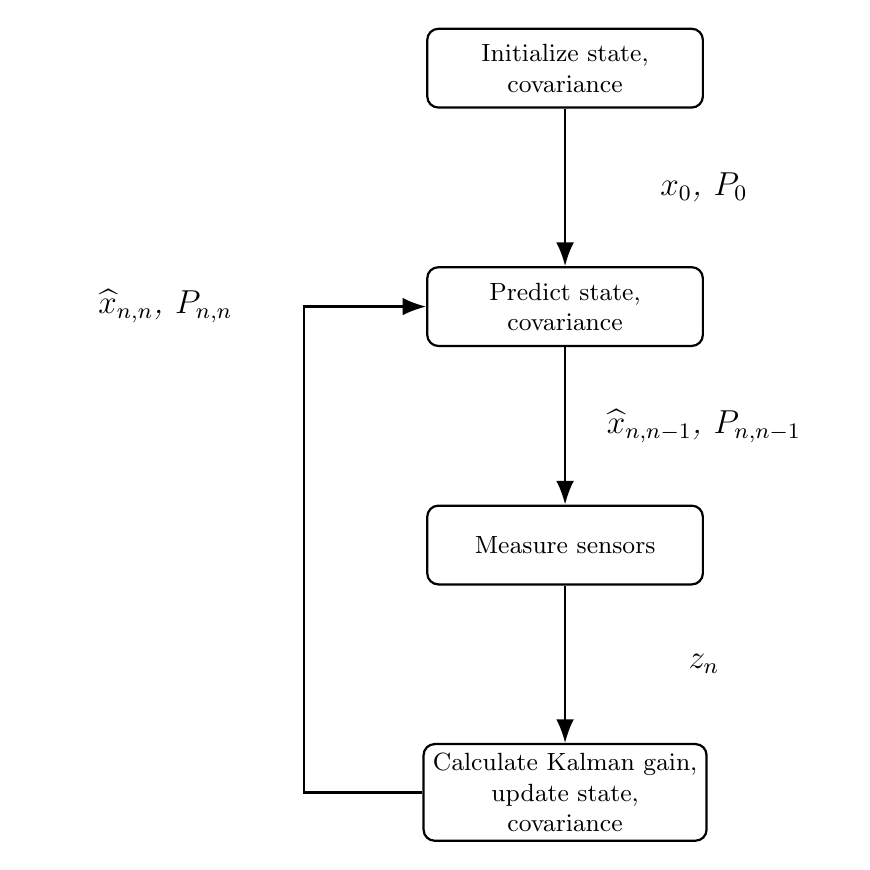
\begin{tikzpicture}[
    node distance=2cm,
    every node/.style={
        rectangle,
        rounded corners,
        draw=black,
        thick,
        minimum width=3.5cm,
        minimum height=1cm,
        align=center,
        font=\small
    },
    arrow/.style={-{Latex[length=3mm]}, thick},
    edgelabel/.style={
        font=\large,
        align=center,
        midway,
        draw=none,
        fill=none
    }
]

% Nodes
\node (init) [align=center] {Initialize state,\\ covariance};
\node (predict) [below=of init, align=center] {Predict state,\\ covariance};
\node (measure) [below=of predict, align=center] {Measure sensors};
\node (update) [below=of measure, align=center] {Calculate Kalman gain, \\ update state,\\ covariance};
% Main flow arrows
\draw[arrow] (init) -- node[edgelabel, right] {\textit{$x_0$, $P_0$}} (predict);

\draw[arrow] (predict) -- node[edgelabel, right] {\textit{$\widehat{x}_{n,n-1}$, $P_{n,n-1}$}} (measure);
\draw[arrow] (measure) -- node[edgelabel, right] {\textit{$z_n$}} (update);

% Loop arrow from update back to predict
\draw[arrow] (update.west) -- ++(-1.5,0) |- node[edgelabel, left, midway] {\textit{$\widehat{x}_{n,n}$, $P_{n,n}$}} (predict.west);

\end{tikzpicture}
\caption{Kalman filter loop}

\label{fig:kalman-loop}
\end{figure}

\begin{table}[htbp !h]
\centering
\caption{Summary of notation and key variables.}
\label{tab:notation}
\begin{tabularx}{\columnwidth}{l X}
\toprule
\textbf{Symbol} & \textbf{Definition} \\
\midrule
$\widehat{x}_{a,b}$  & Estimated state at time step $a$ given information at time $b$ \\
$P_{a,b}$  & Estimated covariance matrix at time step $a$ given information at time $b$ \\
$z_n$               & Measurment at time step $n$ \\
$K_n$               & Kalman Gain at time step $n$ \\
\bottomrule
\end{tabularx}
\end{table}

\clearpage
Unfortunately, their strength in linear systems means they would struggle heavily when applied to a highly nonlinear system like a Baja track. Some extensions to the Kalman filter have been developed to better address nonlinear systems, like the Extended Kalman Filter and the Error-State Kalman Filter. These filters linearize dynamics around the current point by using Taylor series approximations. Our implementation will use an Error-State Kalman filter, as it aims to estimate the error state of the system ($\delta x$) instead of the state ($x$), leading to the linear approximations being more accurate. These filters work as outlined by the diagram below:


\begin{figure}[htbp]
\centering
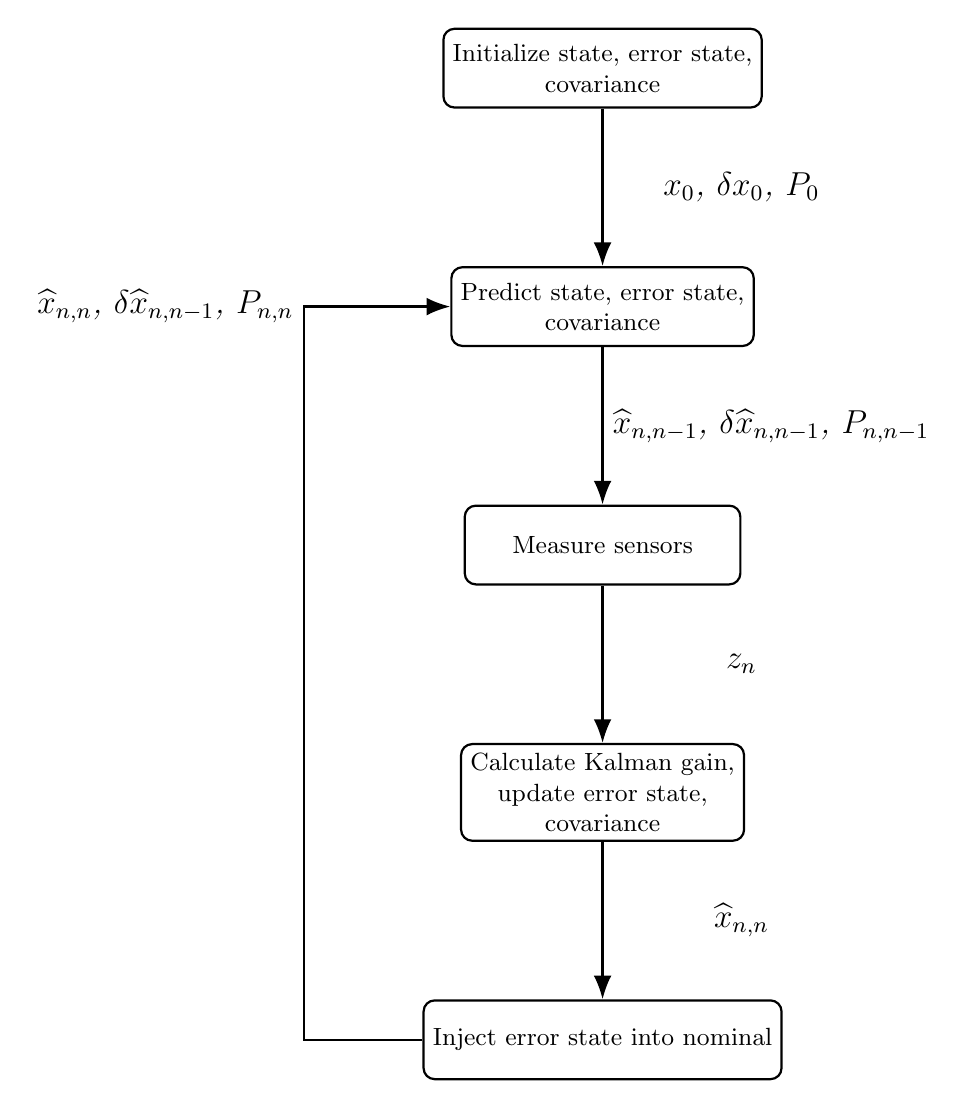
\begin{tikzpicture}[
    node distance=2cm,
    every node/.style={
        rectangle,
        rounded corners,
        draw=black,
        thick,
        minimum width=3.5cm,
        minimum height=1cm,
        align=center,
        font=\small
    },
    arrow/.style={-{Latex[length=3mm]}, thick},
    edgelabel/.style={
        font=\large,
        align=center,
        midway,
        draw=none,
        fill=none
    }
]

% Nodes
\node (init) [align=center] {Initialize state, error state,\\ covariance};
\node (predict) [below=of init, align=center] {Predict state, error state,\\ covariance};
\node (measure) [below=of predict, align=center] {Measure sensors};
\node (update) [below=of measure, align=center] {Calculate Kalman gain, \\ update error state,\\ covariance};
\node (inject) [below=of update, align=center] {Inject error state into nominal};
% Main flow arrows
\draw[arrow] (init) -- node[edgelabel, right] {\textit{$x_0$, $\delta x_0$, $P_0$}} (predict);

\draw[arrow] (predict) -- node[edgelabel, right] {\textit{$\widehat{x}_{n,n-1}$, $\delta \widehat{x}_{n,n-1}$, $P_{n,n-1}$}} (measure);
\draw[arrow] (measure) -- node[edgelabel, right] {\textit{$z_n$}} (update);
\draw[arrow] (update) -- node[edgelabel, right] {\textit{$\widehat{x}_{n,n}$}} (inject);
% Loop arrow from update back to predict
\draw[arrow] (inject.west) -- ++(-1.5,0) |- node[edgelabel, left, midway] {\textit{$\widehat{x}_{n,n}$, $\delta \widehat{x}_{n,n-1}$, $P_{n,n}$}} (predict.west);

\end{tikzpicture}
\caption{Kalman filter loop}

\label{fig:kalman-loop}
\end{figure}


\section{Important vectors}
\subsection{State Vector}
Our state vector must contain four main components:

\begin{itemize}
    \item \textbf{Position}: Location in 3D space
    \[
        \bm{x} = \begin{bmatrix} x \\ y \\ z \end{bmatrix}
    \]

    \item \textbf{Velocity}
    \[
        \dot{\bm{x}} = \begin{bmatrix} \dot{x} \\ \dot{y} \\ \dot{z} \end{bmatrix}
    \]

    \item \textbf{Orientation}: Quaternion $q \in \mathbb{R}^4$
    \[
        \hat{\bm{q}} = \begin{bmatrix} w \\ x \\ y \\ z \end{bmatrix}
    \]

    \item \textbf{Biases}: we must predict biases for both the accelerometer and the gyroscope:
    \[
        \bm{b}_{\text{accel}} = \begin{bmatrix} b_{\text{ax}} \\ b_{\text{ay}} \\ b_{\text{az}} \end{bmatrix}
    \]
    \[
        \bm{b}_{\text{gyro}} = \begin{bmatrix} b_{\text{gx}} \\ b_{\text{gy}} \\ b_{\text{gz}} \end{bmatrix}
    \]
\end{itemize}

Putting this all together, we end up with a $16 \times 1$ vector:
\[
\bm{x}_{\text{state}} =
\begin{bmatrix}
\bm{x} \\
\dot{\bm{x}} \\
\hat{\bm{q}} \\
\bm{b}_{\text{accel}} \\
\bm{b}_{\text{gyro}}
\end{bmatrix}
\]

\subsection{Input Vector}
Our input vector is specified as below:



\begin{itemize}
    \item \textbf{Acceleration}: Acceleration as measured by the IMU
    \[
    \bm{a} = \begin{bmatrix}
        \ddot{x} \\ \ddot{y}\\ \ddot{z} 
    \end{bmatrix}
    \]
    \item \textbf{Angular velocity:} Measured by the gyroscope in the IMU 
    \[
   \bm{\omega} = \begin{bmatrix}
    \omega_x \\ \omega_y \\ \omega_z
   \end{bmatrix}
    \]
\end{itemize}
So in total, 
\[
u = \begin{bmatrix}
    \bm{a} \\ \bm{\omega}
\end{bmatrix}
\]

\subsection{Measurement Vector}
Finally, we have our measurements; the values we check our proposed state against:

\begin{itemize}
    \item \textbf{Steering Position}: Extrapolated steering heading for front wheels from measured steering encoder:
    \[
   \bm{\delta} = \begin{bmatrix}
    \delta_{\text{in}} \\ \delta_{\text{out}}
   \end{bmatrix} 
    \]
    \item \textbf{Wheel Encoders:} Measure the rotations per minute of each wheel: 
    \[
        \bm{n} = \begin{bmatrix}
           n_{\text{fl}} \\
           n_{\text{fr}} \\
           n_{\text{bl}} \\
           n_{\text{br}} \\
        \end{bmatrix}  
    \] 
\end{itemize}

\section{Important Matrices}

\subsection{F \& G}
The $F$ Matrix is the state transition matrix and $G$ is the input transition matrix. They are used as following:
\begin{align}
    x_{n+1,n} = Fx_{n,n} + Gu
\end{align}
$F$ and $G$ combine to give a prediction of the next state given the current state and inputs.

Our Error-State Kalman filter introduces 2 complications:
\begin{itemize}
    \item We are actually focusing our tracking efforts on the error state, not the nominal state.
    \item We are assuming the system is nonlinear. 
\end{itemize}

These complications lead to the following definitions:
\begin{align}
    \widehat{x}_{n+1,n} &= f(\widehat{x}_{n,n}, u) \\
    \widehat{\delta x}_{n+1, n} &= (I + \frac{\partial f_{error}}{\partial \delta x} \Delta t) \widehat{\delta x}_{n,n}
\end{align} 

The second line represents the derivative of a seperate $f$ representing the nonlinear dynamics of the error state. Although these nonlinear dynamics can be hand-differentiated, we will use Python's autodiff as it will remain more accurate especially for later parts of the system and maintains flexibility in case we ever go down a learning-based path. 

\begin{align*}
    
\end{align*}
Our F is defined like this:
\[
\begin{bmatrix}
    0 & I & 0 & 0 & 0\\
    0 & 0 & [\hat{R} \hat{a}]_x & -\hat{R} & 0 \\
    0 & 0 & -[\hat{w}]_x & 0 & -\hat{R} \\
    &\dots &0& \dots \\
    &\dots &0& \dots \\
\end{bmatrix}
\]
\section{H}
We formalize the concept of "conditioning our state on our observations" with the concept of Kalman gain, denoted as $K_n$. This quantity represents how much we trust new measurements, and how much we'll factor them into our updated state. Kalman gain for a linear Kalman filter is defined as:
\[
K_n = P_{n,n-1}H^T \cdot (H P_{n,n-1}H^T + R_n)^{-1}
\]
In scalar form, we can more intuitively write it as:
\[
K_n = \dfrac{P_{n,n-1}}{P_{n,n-1}+R_n}
\]
and we update our state with: 
\[
\widehat{x}_{n,n} = \widehat{x}_{n,n-1} + K_n(z_n - H\widehat{x}_{n,n-1})
\]

\begin{table}[htbp !h]
\centering
\caption{Matrix and variable notation.}
\label{tab:matrices}
\begin{tabularx}{\columnwidth}{l X}
\toprule
\textbf{Symbol} & \textbf{Definition} \\
\midrule
$H$  & Maps state vector to expected measurement values\\
$R$  & Sensor noise matrix \\
\bottomrule
\end{tabularx}
\end{table}
In scalar form, a Kalman gain of $1$ correlates to fully trusting your measurement, and $0$ vice versa. Let's look at the end behavior to get some intuition:

As $P \gg R$, $K \lim\to 1$. This physically means that your uncertainty on your state is extremely high, and so then regardless of how much noise our sensors have we trust the measurement 100\%. This is commonly used near the beginning of the estimation process when we initialize a guess of the system.
As $R \gg P$, $K \lim \to 0$. This correlates with extremely high sensor noise, meaning we take our previous prediction with no weight on the new measurement.
The more complex form does a similar process with some intermediary steps like projecting the covariance matrix into the measurement space, but the general idea remains the same. 

The H matrix is much more granular than the F matrix, and operates directly on component vectors.

\end{document}